\documentclass[%
 reprint,
%superscriptaddress,
%groupedaddress,
%unsortedaddress,
%runinaddress,
%frontmatterverbose, 
%preprint,
%preprintnumbers,
%nofootinbib,
%nobibnotes,
%bibnotes,
 amsmath,amssymb,
 aps,
%pra,
%prb,
%rmp,
%prstab,
%prstper,
%floatfix,
]{revtex4-2}

\bibliographystyle{pre}
\usepackage{graphicx}% Include figure files
\usepackage{dcolumn}% Align table columns on decimal point
\usepackage{bm}% bold math
\usepackage{color}
%\usepackage{appendix}
\newcommand{\ericblue}[1]{{\color{blue}#1}} % change
\newcommand{\yjred}[1]{{\color{red}#1}} % change

%\usepackage{hyperref}% add hypertext capabilities
%\usepackage[mathlines]{lineno}% Enable numbering of text and display math
%\linenumbers\relax % Commence numbering lines

%\usepackage[showframe,%Uncomment any one of the following lines to test 
%%scale=0.7, marginratio={1:1, 2:3}, ignoreall,% default settings
%%text={7in,10in},centering,
%%margin=1.5in,
%%total={6.5in,8.75in}, top=1.2in, left=0.9in, includefoot,
%%height=10in,a5paper,hmargin={3cm,0.8in},
%]{geometry}

\begin{document}

\title{Effects of Polydispersity on the Plastic Behaviors of Dense 2D Granular Systems Under Shear}
\author{Yonglun Jiang}
% \altaffiliation[Also at ]{Physics Department, XYZ University.}%Lines break automatically or can be forced with \\
%\author{Second Author}%
\affiliation{Department of Physics, Emory University,
Atlanta, GA 30322, USA}
\email{yjia249@emory.edu, erweeks@emory.edu}

\author{Daniel M. Sussman}
\affiliation{Department of Physics, Emory University,
Atlanta, GA 30322, USA}

\author{Eric R. Weeks$^*$}
\affiliation{Department of Physics, Emory University,
Atlanta, GA 30322, USA}
%\email{erweeks@emory.edu}

\date{\today}% It is always \today, today,
             %  but any date may be explicitly specified

\begin{abstract}
We study particle-scale motion in sheared highly polydisperse amorphous materials, in which the largest particles are as much as ten times the size of the smallest. We find strikingly different behavior from the more commonly studied amorphous systems with low polydispersity.  In particular, analysis of the nonaffine motion of particles reveals qualitative differences between large and small particles: the smaller particles have dramatically more nonaffine motion, which is induced by the presence of the large particles.  We characterize how the nonaffine motion changes from the low- to high-polydispersity regimes.  We further demonstrate a quantitative way to distinguish between ``large'' and ``small'' particles in systems with broad distributions of particle sizes.  A macroscopic consequence of the nonaffine motion is a decrease in the energy dissipation rate for highly polydisperse samples, which is due both to a geometric consequence of the changing jamming conditions for higher polydispersity and to the changing character of nonaffine motion. 
\end{abstract}

%\keywords{Suggested keywords}%Use showkeys class option if keyword
                              %display desired
\maketitle

%\tableofcontents

\section{Introduction}
\label{intro}

Amorphous materials are common, ranging from glasses to emulsions, foams, granular media, cement pastes, food products, and more.  These materials are often composed of mixtures of various sizes of particles.  Much prior work has studied the flow of amorphous materials using model systems with low polydispersity, which is to say, mixtures of particles of fairly similar sizes
\cite{liu96,mason97emulsions,hebraud97,petekidis02,schall07,chen10,vasisht18,tsai21,yamamoto97,falk98,teitel07,utter08,lemaitre09,manning11,cubuk15,hassani19,losert00,patinet2016connecting}.  However, many natural materials are highly polydisperse, with particle sizes varying by factors of ten or more, which impacts the flow of glaciers \cite{haeberli06}, landslides and avalanches \cite{pitman05}, soil \cite{or02}, mud \cite{besq03}, cement \cite{rosquoet03}, and food products \cite{taylor09}. Computational studies have also increasingly relied upon moderately polydisperse model glassformers, where manipulating particle sizes allows studies of equilibrium glass configurations at unusually low temperatures~\cite{ninarello2017models,berthier2017configurational,brito2018theory,kapteijns2019fast}. These natural and model systems with large polydispersity are complex and spatially heterogeneous, and it is hard to extract general principles.  The goal of this paper is to examine the role of the particle size distribution in sheared materials and, in so doing, bridge between simple model systems with low polydispersity and complex highly polydisperse real-world materials.


Polydispersity leads to interesting physics.  For example, polydisperse hard spheres can phase separate into multiple crystalline phases \cite{sollich10}.  Polydispersity can lead to new phases for active matter systems \cite{kumar21}.  An experimental study of polydisperse colloidal glasses found that different particle sizes had different dynamics and local environments \cite{heckendorf17}.  Diffusion of tracers in porous materials becomes anomalous when the porous medium is highly polydisperse \cite{cho12}.  Force chains in granular materials become dramatically more heterogeneous in more polydisperse systems \cite{nguyen14,nguyen15,cantor18}.  The viscosity of particulate suspensions strongly depends on polydispersity \cite{pednekar18}, varying by orders of magnitude for constant volume fraction of particles \cite{chong71}.  These studies highlight how new physics can emerge from complex particle size distributions, but prior work studying sheared amorphous materials typically downplays the role of particle size distributions.  Experiments and simulations of sheared amorphous materials often use slightly polydisperse samples to inhibit the formation of crystalline structures:  for example, using two distinct sizes with size ratio $O(1)$ \cite{yamamoto97,falk98,teitel07,utter08,lemaitre09,manning11,cubuk15,hassani19} or experiments using nominally single component systems with small intrinsic polydispersity \cite{liu96,mason97emulsions,hebraud97,petekidis02,schall07,chen10,vasisht18,tsai21}.  These studies led to insights such as the importance of non-affine motion in sheared disordered materials \cite{falk98,utter08,schall07}, but generally treat the amorphous system as homogeneous.  Exceptions to the assumption of homogeneity exist; for example studies show that ``soft spots'' in amorphous materials are more likely to exhibit particle rearrangements under shear \cite{manning11}, although even in these analyses, it is common to focus on identifying soft spots centered only on larger particles in a bidisperse mixture \cite{cubuk15,schoenholz16,bapst2020unveiling}. It is far from clear that many of the methods used to identify these disordered ``defects'' in the solid will generalize to highly polydisperse samples, or that particles of different sizes within a highly polydisperse sample will even qualitatively show similar non-affine behavior under shear.  Indeed, a confocal microscopy study of a sheared highly polydisperse emulsion showed qualitative differences in the motion of large and small droplets \cite{clararahola15}.


In this paper we show that highly polydisperse 2D amorphous systems under shear are qualitatively different from systems of low polydispersity. We show that large particles behave qualitatively differently from small particles; we demonstrate how to quantify which particles are ``large'' and ``small''; and we show how these effects appear as the particle size distribution broadens.  Additionally, our results show that the largest particles strongly influence nearby particle rearrangements, suggesting that previously studied soft spots (e.g. \cite{manning11,cubuk15,schoenholz16,bapst2020unveiling,boattini2021averaging}) will be different in character -- and easier to identify -- in highly polydisperse materials.

\section{Computational Methods}

We simulate the two-dimensional Durian bubble model \cite{durian95} using the non-mean-field version introduced in Ref.~\cite{tewari99}, in which particles have repulsive contact forces and experience viscous forces from neighboring particles.  Two particles with interparticle distance $r_{ij}$ smaller than the sum of their radii $R_i+R_j$ overlap.  Overlapping particles experience a repulsive force:
\begin{equation}
    \label{equation_1}
    \Vec{F}_{ij}^{\rm repulsive}=F_0 (1-\frac{\vec{r}_{ij}}{|R_i+R_j|})\hat{r}_{ij}
\end{equation}
and also a viscous force:
\begin{equation}
    \label{equation_2}
    \Vec{F}_{ij}^{\rm viscous}=b(\Vec{v}_i-\Vec{v}_j).
\end{equation}
The repulsive force acts in directions to push the two particles apart, and the viscous force acts on each bubble to try to bring their velocities $\vec{v}_i$ and $\vec{v_j}$ into agreement.  $F_0=1$ and $b=1$ are constants indicating the relative strength of the two forces.  The dependence of the repulsive force on $R$ means that larger particles are effectively softer.  Given that the bubbles are massless, the forces on each bubble must sum to zero, which results in equations that can be solved for each bubble's velocity $\vec{v}_i$.  This then is a set of differential equations which are solved using fourth order Runge-Kutta.  Other computational details are as given in Ref.~\cite{hong17}.

We consider a variety of truncated exponential size distributions, $P(R) \sim \exp(-R/\lambda)$ where $R$ is the radius, considered over the domain $R_{\rm min} \leq R \leq R_{\rm max} \equiv \alpha R_{\rm min}$. We study systems in which $\alpha$, which characterizes the width of the distribution, ranges from 2 to 10. The decay constant $\lambda$ is set to $R_{\rm min}$. We take $\langle R \rangle$ as our unit of length, and we nondimensionalize time by the microscopic relaxation time (based on the inter-particle spring constant and viscous damping forces \cite{durian95}). We will compare the properties  of these exponentially distributed systems with a standard bidisperse mixture composed of equal numbers of particles whose size ratio is $1 : 1.4$. All of these distributions can be characterized by their polydispersity $\delta$, defined as the standard deviation of $P(R)$ divided by $\langle R \rangle$; the values of $\delta$ and $R_{min}$ are given in Table~\ref{tab:size}. 

We shear these systems in square boxes with length $L$ using Lees-Edwards boundary conditions. We keep $\frac{L}{\langle R \rangle} = 100$ constant which guarantees that $L$ is at least $20R_{\rm max}$  for our systems. The area fraction $\phi$ is 0.93, which is well above the jamming transition point ($\phi_J= 0.84 - 0.86$ for our particle size distributions).  We wish to shear at a slow rate, but nonetheless fast enough that the computational time is not excessive.  The rheological behavior of two of our systems is shown in Fig.~\ref{fig:hb}, and we pick our nondimensional strain rate to be $\dot{\gamma} = 10^{-4}$ as a compromise where the total stress is less than twice the yield stress, and the computational speed is adequate.  We simulate the shear at least up to strain $\gamma=10$ to ensure enough statistics; an initial transient response for $\gamma < 0.2$ is discarded before analysis.   We will focus most of our discussion on the $\alpha=10$ (maximally polydisperse) systems of $2500$ particles and the bidisperse systems of $3098$ particles. A snapshot of a portion of the polydisperse system under shear is shown in Fig.~\ref{fig:sample_example}(a).


\begin{figure}[ht]
    \centering
    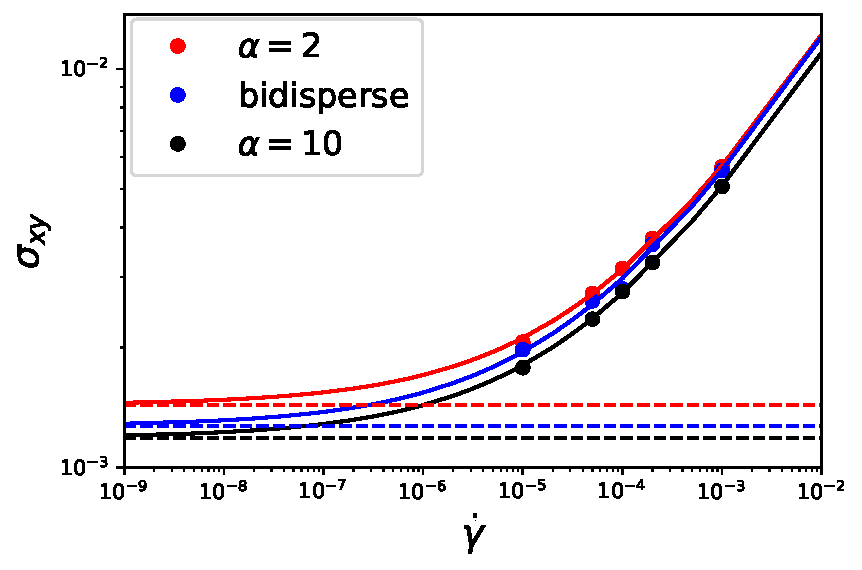
\includegraphics[width=8cm]{hb_exp10_bi_stressxy123022.pdf}
    \caption{Stress as a function of strain rate for the low polydispersity sample ($\alpha=2$, top data), bidisperse sample (middle data), and the highly polydisperse sample ($\alpha=10$, bottom data).  The fit lines are to the Herschel-Buckley formula, $\sigma = \sigma_0 + K \dot{\gamma}^{0.4}$.  The horizontal dashed lines indicate the yield stresses $\sigma_0$.  The simulations analyzed in the remainder of our paper are at $\dot{\gamma}=10^{-4}$.}  
    \label{fig:hb}
    \vspace*{-12pt}
\end{figure}

\begin{table}
    \centering
    \begin{tabular}{c|c|c|c|c|c}
    $\alpha$ & $10$ & $5$ & $4$ & $3$ & $2$ \\
    \hline
    $R_{min}$ & 0.50 & 0.52 & 0.54 & 0.59 & 0.71 \\
    %\hline
    $\delta$ & 0.50 & 0.43 & 0.39 & 0.31 & 0.20
    \end{tabular}
    \caption{$R_{min}$ and polydispersity $\delta$ for the exponential size distributions we use. $R_{max}=R_{min} \alpha$. Note that $R_i=0.83,1.17$ in our bidisperse system ($\delta=0.17$).}
    \label{tab:size}
\end{table}


\section{Results}

\subsection{Nonaffine motion of individual particles}

\begin{figure}[ht]
    \centering
    \includegraphics[width=8.6cm,bb= 20 120 580 350]{newfig1.eps}
    \caption{(Color online). Panel (a) shows a snapshot of a system with an exponential size distribution, with the particle size ratio $R_{\max}/R_{\rm min}= \alpha = 10$. Pink arrows indicate the total displacements of particles for a strain interval of $0.005$.  Panel (b) sketches the mean flow pattern around large particles under the applied shear strain.  
    }
    \label{fig:sample_example}
    \vspace*{-12pt}
\end{figure}

We examine particle motion over small strain intervals $\Delta \gamma = 0.005$, an interval over which particles do not rearrange dramatically. To characterize the behavior of individual particles, we consider the non-affine component of motion by subtracting off the mean (affine) flow: $\Delta \vec{r}_{{\rm NA},i} = \Delta \vec{r}_{i} - \Delta \gamma \, y_{i}  \hat{x}$, where for particle $i$, the first term on the right hand side (RHS) is the real motion over $\Delta \gamma$, and the second term on the RHS is the affine motion imposed by the simulation, where $\hat{x}$ is the velocity direction and $y_{i}$ is the position in the gradient direction. Local rearrangements cause deviations from purely affine motion, as seen in Fig.~\ref{fig:sample_example}(a):  were the motion entirely affine, all arrows would be horizontal. 

\begin{figure}[ht]
    \centering
    \includegraphics[width=8cm]{ndr_r_alldata_080323.eps}
    \caption{Averaged $\Delta \vec{r}_{\rm NA,i}^{\,2}$ versus particle radius $R$ for systems with different size distributions.  From top curve (blue) to bottom (purple) the symbols symbols correspond $\alpha = 2, 3, 4, 5,$ and $10$. Diamonds are for the bidisperse particle size distribution. Inset shows measured nonaffine motion field $\langle \Delta r_{\rm NA} \rangle(x,y)$ around reference particles with $2 \leq R_i \leq 2.8$ indicated by the two concentric circles.  For the region $R_i < 2.8$, arrows are only drawn where sufficient data exists.  Data are for the system with $\alpha=10$.}
    \label{fig:ndr_radius}
    \vspace*{-12pt}
\end{figure}

To understand how nonaffine motion depends on particle size, we calculate the mean $\Delta \vec{r}_{\rm NA,i}^{\,2}$ as a function of particle size $R$, shown in Fig.~\ref{fig:ndr_radius}.  On average $\Delta \vec{r}_{\rm NA,i}^{\,2}$ decreases with $R$ for all systems, including the bidisperse system; this agrees qualitatively with previous observations in polydisperse emulsions under cyclic shear \cite{clararahola15}.  Figure \ref{fig:ndr_radius} shows that large particles are more likely to follow the affine shear flow, whereas small particles will have more shear-induced diffusivity. A simple explanation is that large particles have more neighbors than small ones. The influence of these neighbors on the motion of the large particles on average cancel with each other, which results in the larger particles having smaller magnitude of $\Delta \vec{r}_{\rm NA,i}$.  Note that the bidisperse results also match to the family of curves, showing measurably different $\Delta \vec{r}_{\rm NA,i}^{\,2}$ values for small and large particles.

These results reveal the following microscopic picture of motion near the large particles.  Large particles are ``strong'' and have less nonaffine motion; they are more likely to follow the affine imposed shear flow.  In the reference frame co-moving with the affine velocity of a large particle, this relative immobility causes the ``weaker'' small particles to detour around the larger particles, as sketched in Fig.~\ref{fig:sample_example}(b).  Examining trajectories of individual particles reveals motions that qualitatively match the sketch of Fig.~\ref{fig:sample_example}(b) (data not shown).

\subsection{Mean nonaffine flow fields}

To understand how large particles perturb the flow we calculate the average non-affine flow field around particles of different sizes. We average the non-affine motion $\langle \Delta \vec{r}_{{\rm NA},j} \rangle$ of all particles $j$ at a specific position $(x,y)$ relative to the center of a reference particle $i$. We bin the relative position $(x,y)$ with tolerance $\delta x = \delta y = 0.1$. We then average that field over all reference particles $i$ with radii $R_i$ in a specific range to get better statistics yielding $\langle \Delta \vec{r}_{{\rm NA}}\rangle(x,y)$.  In Fig.~\ref{fig:ndr_radius} inset we show this field for particles with $2.0 \leq {R}_i \leq 2.8$.  The top left and bottom right, relative to the reference particle, are referred to as the ``compressive directions'' as the imposed affine flow tries to push neighboring particles toward the reference particles \cite{batchelor_determination_1972,bergenholtz02}.  This affine push is resisted by the large reference particle, resulting in outward-pointing non-affine motion.  Likewise, the regions at the top right and bottom left are referred to as the ``extensional directions'' in terms of the background flow, and the non-affine motion is inward.  Adding the background affine shear flow to the nonaffine flow field yields the qualitative sketch of Fig.~\ref{fig:sample_example}(b).  This non-affine motion field illustrates the importance of relative positions in the polydisperse sample.

\begin{figure}
    \centering
    \includegraphics[width=8cm]{ndrfield_020922.eps}
    \caption{Color field of $\Delta \vec{r}_{\rm NA,i} \cdot \hat{r}$; the dot product with $\hat{r}$ selects for components of the motion that are outward (light red) or inward (dark blue), as indicated by the color bar. From left to right, the top two panels are size ranges $R_i = 0.80-0.84$ and $2.0-2.8$ using data from $\alpha=10$ system. The bottom two panels are from the bidisperse system for the small (lower left) and large (lower right) particles.}
    \label{fig:ndr_field}
    \vspace*{-20pt}
\end{figure}

Figure \ref{fig:ndr_field} shows four examples of the $\hat{r}$ component of $\Delta \vec{r}_{\rm NA}(x,y)$ to demonstrate how the field differs with different
reference particle sizes.  The top two panels are data from the broadest particle size distribution, examining the flow around smaller (top left) and larger (top right) particles.  For comparison, the bottom two panels are for the bidisperse distribution. We highlight that in this system a finite far-field can be identified and whose sign in the top left panel is opposite to the field in the top right panel.  The far field is less obvious in the bottom two panels, although still present to a small degree as will be quantified below.

The interpretation of the top panels of Fig.~\ref{fig:ndr_field} is that large particles are strong, move more affinely, and force the other particles to detour around them.  For the smaller reference particles, the influence of the reference particle is clearly different. Neighboring particles at the surface of any reference particle (large or small) can have minimal center-to-center distances with the reference particle only if they are themselves small particles.  Thus the region immediately at the surface of a reference particle is composed of small particles and at the surface all cases in Fig.~\ref{fig:ndr_field} look the same: an outward non-affine motion along the compressive direction, and inward non-affine motion along the extensional direction.  However, farther away from small reference particles, the size of neighboring particles can be significantly larger than the reference particle.  These small reference particles are weaker and more likely to be moved nonaffinely by their neighboring particles.  Thus, the inward moving (dark blue) colors around the small reference particle along the compressive directions reflect that, on average, the small reference particle is being pushed away from the neighbors along these directions.  In other words, the non-affine motion pattern around large reference particles, as seen in Fig.~\ref{fig:ndr_field}(top right), is precisely because the large reference particles are larger than many other particles; and the pattern around smaller reference particles is qualitatively different precisely because they are smaller than many other particles.

To verify this assertion, we quantify the behavior of $\Delta \vec{r}_{\rm NA}(x,y) \cdot \hat{r}$ by least squares fitting the field data to $A_2(R_i,r)\sin{2\theta}$. That is, we switch from $(x,y)$ to $(r,\theta)$, taking advantage of the symmetry of Fig.~\ref{fig:ndr_field} to express the magnitude of the flow in terms of the prefactor $A_2(R_i,r)$. Higher frequency terms, of the form  $\sin{n\theta}$, have prefactors at least an order of magnitude smaller than $A_2$ and are thus ignored. The results for $A_2(R_i,r)$ for several reference droplet radii $R_i$ are shown in Fig.~\ref{fig:far_a2}(a), showing an obvious dependence of $\Delta \vec{r}_{\rm NA}$ on size. For the largest reference particles (${R}_i=5$, the purple curve) $A_2$ is negative for all distances $r$ from the reference particles.  This negative $A_2$ indicates that the large particles are strong, and cause the average flow field sketched in Fig.~\ref{fig:sample_example}(b) and quantified in Fig.~\ref{fig:ndr_field}(top right).  The shape of $A_2$ gradually changes with decreasing ${R}_i$. For the smallest reference particles ($R_i=0.5$, the  pink curve), $A_2$ is positive over most of the range, with a small exception at the smallest $r$.  This confirms that these particles are weak, and are the ones whose motion is most often perturbed by the larger particles, quantifying what is seen in Fig.~\ref{fig:ndr_field}.  For the bidisperse case, the two $A_2$ curves for the two sizes oscillate [Fig.~\ref{fig:far_a2}(a) inset].  The oscillations reflect the pair correlation function and match the rings visible in the bottom two panels of Fig.~\ref{fig:ndr_field}.

\begin{figure}
    \centering
    \includegraphics[width=8cm]{rstar_a2r_081923.eps}
    \caption{(a) Prefactor characterizing the non-affine field, $A_2$, versus distance, $r$, for several reference particle sizes in the $\alpha=10$ system.  The inset shows $A_2$ for the bidisperse system, where black (grey) curve corresponds to the smaller (larger) particles. (b) $\langle A_{2,far} \rangle$ versus $R$ curves for three systems. Color indicates size spans for $\alpha = 10, 5,$ and 3; [colors matching Fig.~\ref{fig:ndr_radius}(a)] and the open diamonds correspond to the bidisperse system. Solid lines are quadratic fits to guide the eye. The crossing zero point at each solid line is defined as $R^{\ast}$. The scatter at large $R$ results from lack of statistics given that large particles are rare.}
    \label{fig:far_a2}
    \vspace*{-10pt}
\end{figure}

We wish to understand how these results depend on the size of the reference particles. Here we focus on the far field:  in some cases $A_2>0$ $(<0)$ for large $r$ indicating weak (strong) particles.  We quantify the far field by calculating the average $\langle {A_2}(r) \rangle_r$ over $R_i + 6 \leq r \leq 40$; our results are not sensitive to this choice.  The qualitative results discussed above are confirmed in  Fig.~\ref{fig:far_a2}(b): the flow pattern for non-affine motion differs in sign for small reference particles as compared to large reference particles.

These results answer two interesting questions.  First, for a given size distribution, how do we distinguish between ``large'' and ``small'' particles? We propose $\langle A_{2,{\rm far}}(R^*) \rangle = 0$ as the criteria separating the two classes of particles.  For the broad ($\alpha=10$) particle size distribution we find ${R}^* = 1.7 \pm 0.1$. Second, how does this length scale depend on the particle size distribution?  Figure~\ref{fig:delta}(a) shows $R^*$ as a function of the polydispersity $\delta$ of the particle size distributions.  $R^*$ grows for broader particle size distributions.  Intriguingly, in our systems the relative fraction of particles with $R_i > R^*$ decreases from 43\% to only 8\% from our narrowest to broadest size distributions. 


\begin{figure}
    \centering
    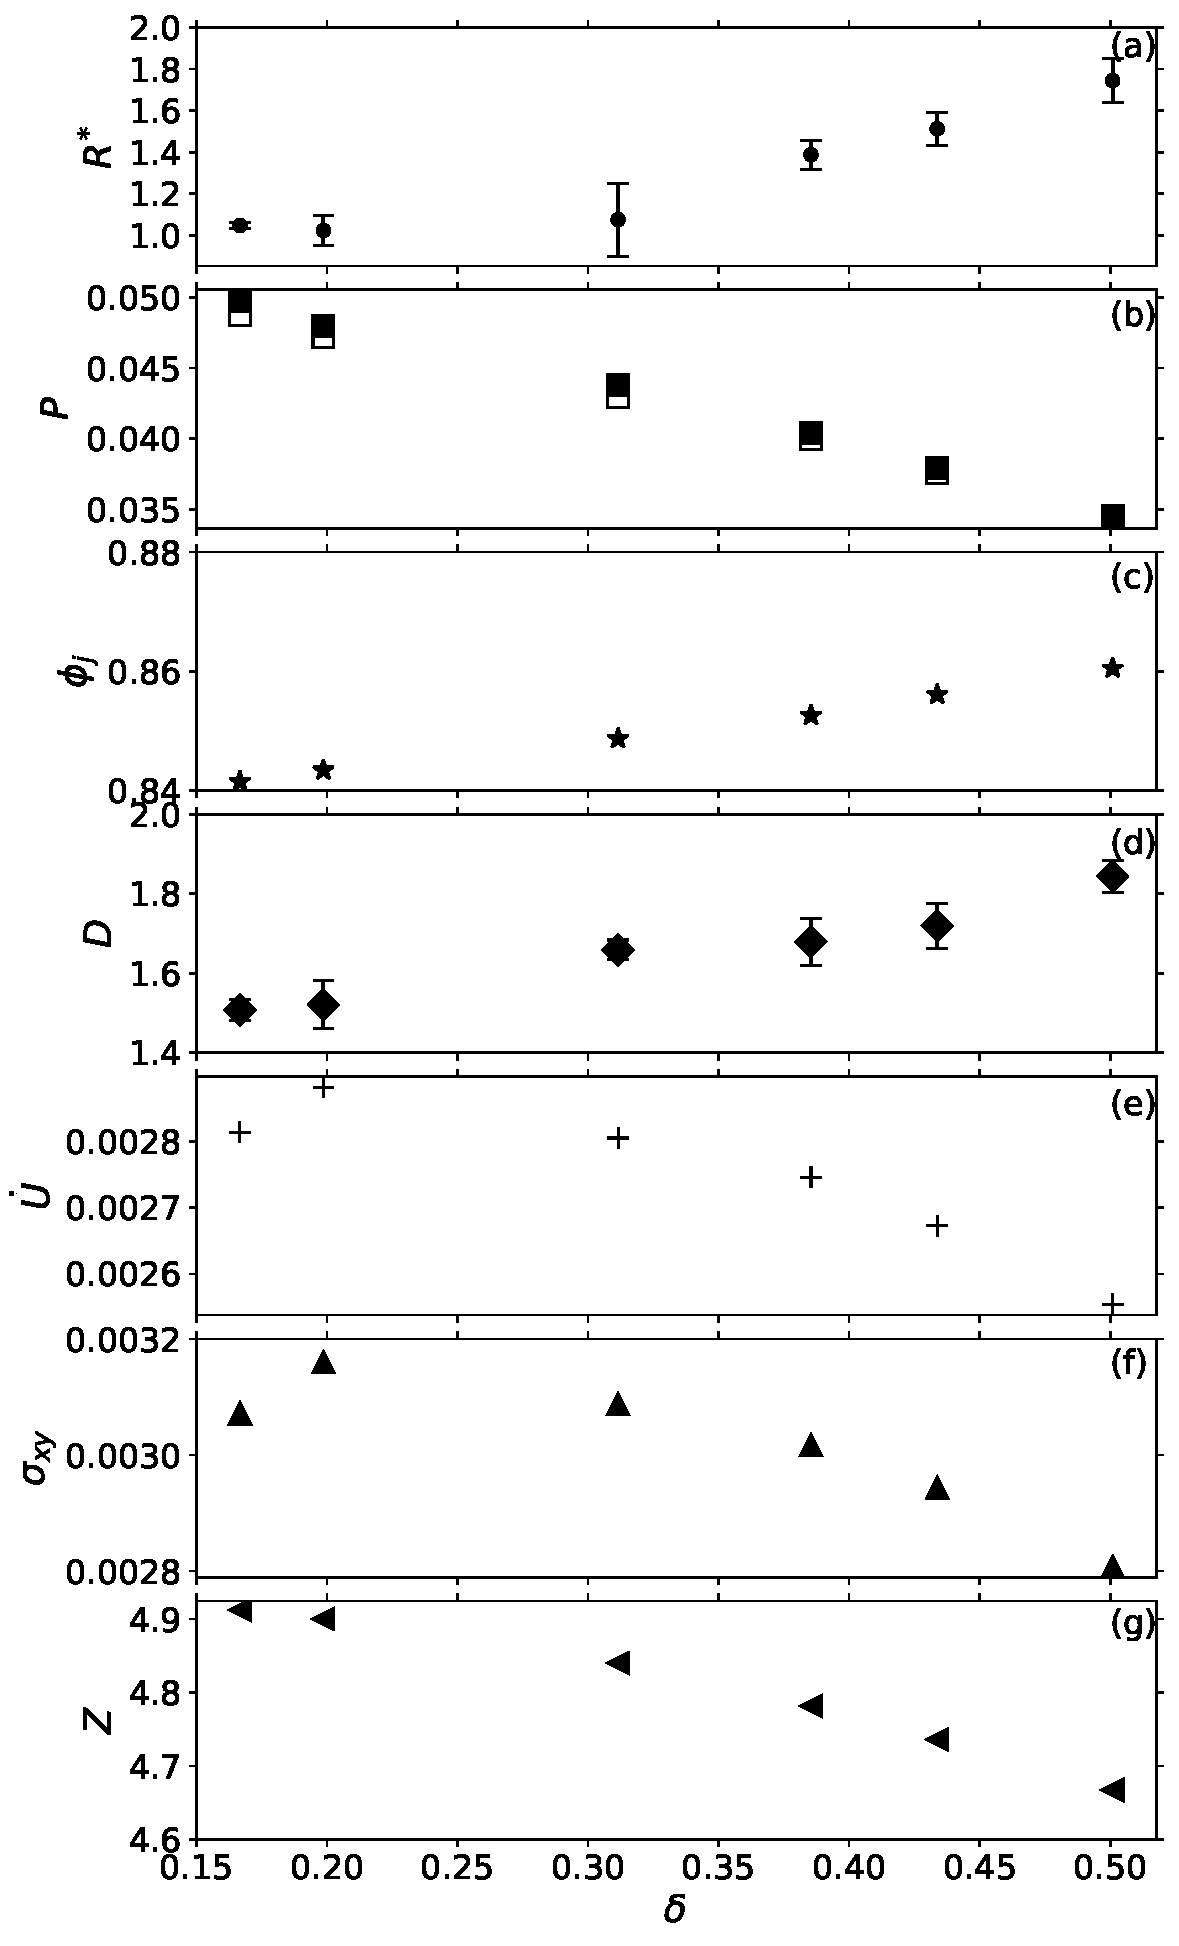
\includegraphics[width=8cm]{quantities_delta101123.pdf}
    \caption{This figure shows a variety of quantities as a function of the polydispersity $\delta$; in all plots the smallest value of polydispersity ($\delta=0.17$) corresponds to bidisperse data, the second smallest ($\delta=0.20$) corresponds to the distribution with $r_{\max}/r_{min} = \alpha = 2$, and the highest ($\delta = 0.50$) corresponds to $\alpha=10$.  Where shown, the error bars indicate uncertainty based on five independent simulations.  Where not shown, the uncertainties are smaller than the symbol size. 
    (a) $R^{\ast}$ obtained from $A_2$ against the polydispersity [Fig.~\ref{fig:far_a2}(b)].  (b) Pressure of the sheared system (filled symbols) and of the unsheared system (open symbols).  (c) Jamming area fraction $\phi_J$ (recall that the simulations are performed at $\phi = 0.93 > \phi_J$).  (d) Mean effective particle diffusivity $D$ measured from $\langle \Delta y^2 \rangle = 2 D \Delta \gamma$ in the limit of $\Delta \gamma > 1$ (see Fig.~\ref{fig:strainintervalcheck}). (e) Energy dissipation rate $\dot{U}$.  (f) Shear stress $\sigma_{xy}$ at our strain rate $\dot{\gamma} = 10^{-4}$.  (g) Mean contact number $Z$.}
    \label{fig:delta}
    \vspace*{-10pt}
\end{figure}


\subsection{Energy dissipation depends on polydispersity}

These results have implications for a macroscopic property of these samples:  the total energy dissipation rate is lower for the highly polydisperse samples.  In our model, the power supplied by external driving is dissipated through the viscous force as 
\begin{equation}
    \sigma \dot{\gamma} A = \frac{1}{2} \sum_{i > j} (\vec{v_i}-\vec{v_j})^2,
\end{equation}
where $\sigma$ is the shear stress, $A$ is the area, and the sum is over all pairs of particles $(i,j)$ in contact \cite{tighe10}. 
The dissipation rate decreasesby 12.4\% as the size distribution is changed from $\alpha=2$ to $\alpha=10$.


\begin{table}
    \centering
    \begin{tabular}{|c|c|}
    \hline
    quantity & change as $\alpha = 2 \rightarrow 10$\\
    \hline
    $D$ & $+21.3\%$ \\
    $p$ & $-28.0\%$ \\
    $p^{*}$ & $-27.0\%$ \\
    $Z$ & $-4.75\%$ \\
    $\dot{U}$ & $-12.4\%$\\
    $\sigma_{xy}$ & $-12.5\%$ \\
    $\sigma_0$ & $-17.3\%$ \\
    $\Delta \sigma$ & $-8.42\%$ \\
    \hline
    \end{tabular}
    \caption{This table shows how quantities change when comparing the $\alpha=10$ system to the $\alpha=2$ system, that is, $(X(\alpha=10)-X(\alpha=2))/X(\alpha=2)$.  The quantities are diffusivity $D$, pressure $p$, pressure without shear $p^{*}$, energy dissipation rate $\dot{U}$, average contact number per particle $Z$, shear stress $\sigma_{xy}$, yield stress $\sigma_0$, and $\Delta \sigma = \sigma_{xy} - \sigma_0$. }
    \label{tab:percents}
\end{table}



As the dissipation derives directly from velocity differences $(\vec{v_i}-\vec{v_j})^2$ between contacting particles, the decreasing dissipation rate can be related to nonaffine motion.  There are two competing effects.  First, note that the velocities can be decomposed into affine and nonaffine components.  Independent of the polydispersity, the nonaffine component $(\vec{v_{NA,i}}-\vec{v_{NA,j}})^2$ constitutes about 94\% of the total dissipation (the affine component $(\vec{v_{A,i}}-\vec{v_{A,j}})^2$ constitutes around 6\%, and cross-terms involving $\vec{v_A}$ and $\vec{v_{NA}}$ are negligible).  Figure~\ref{fig:ndr_radius}(a) highlights that there is a broader range of $v_{NA}$ for the more polydisperse systems. Thus, $\langle (\vec{v_{NA,i}}-\vec{v_{NA,j}})^2 \rangle$ is observed to be larger for higher polydispersity:  on average each contact dissipates more energy, 10\% more for $\alpha=10$ as compared to $\alpha=2$.  (The affine component dissipation also increases with increasing polydispersity.)  Second, given that we keep the system size $L/\langle R \rangle$ constant between the different simulations, highly polydisperse samples have fewer particles and thus fewer contacts:  21\% fewer contacts for $\alpha=10$ as compared to $\alpha=2$.  The product of the mean dissipation per contact and the number of contacts results in an overall decrease of the total dissipation decreases as the polydispersity increases, consistent with prior work \cite{pednekar18}.

An alternate view of the energy dissipation stems from a macroscopic, geometrical perspective.  As noted above, the energy dissipation rate is $\sigma \dot{\gamma} A$.  Figure \ref{fig:hb} shows that at our stress rate $\dot{\gamma} =10^{-4}$, the stress is partially due to the yield stress (accounting for 45.5\% of the total stress at the lowest polydispersity) and partially due to a rate-dependent term (accounting for the remainder of the stress).  The yield stress, being a quantity measured as $\dot{\gamma} \rightarrow 0$, is purely dependent on geometry and in particular is a function of $\phi-\phi_J$, the area fraction compared to the jamming transition area fraction. As seen in Fig.~\ref{fig:delta}(c), $\phi_J$ increases with increasing polydispersity; thus the yield stress drops as given in Table \ref{tab:percents}.  The rate-dependent component of the stress also drops, as given by the entry for $\Delta \sigma$ in the Table.  Thus the change in total stress $\sigma$ is $(-17.3\% \times 0.455) + (-8.42\% \times (1-0.455)) = -12.5\%$, showing that the data in Table \ref{tab:percents} correctly account for the decrease in $\sigma$ and thus the decrease in energy dissipation rate $\dot{U}$.  In particular, the geometric component of the decreasing energy dissipation rate is almost twice as large as the non-affine ($\dot\gamma$ dependent) component of the decrease; nonetheless, both components are significant.




\subsection{Dependence on strain interval}

Above we use a strain interval $\Delta \gamma= 0.005$ to calculate the nonaffine motion.  This choice is based the mean square displacement of particles, as shown in Fig.~\ref{fig:msd}.  The system exhibits ballistic motion ($\langle \Delta y^2 \rangle \sim \Delta \gamma^2$) until $\Delta \gamma \sim 10^{-2}$.  This suggests that motion up to strain increment of 0.005 is within individual coherent rearrangement events (the relaxation of a plastic event, for example) and then motion over longer strain intervals is more uncorrelated, leading to a random walk of particles in space.  Our choice of $\Delta \gamma= 0.005$ ensures that particles have displacements well beyond numerical precision, while not yet (on average) having undergone more than one rearrangement motion.

\begin{figure}
    \centering
    \includegraphics[width=8cm]{msd_y_noboundary_exp10_100622.eps}
    \caption{Mean squared displacement in the gradient direction as a function of strain interval $\Delta \gamma$ for the $\alpha=10$ system. The left dashed line has a slope of 2 indicating ballistic motion, and the right dashed line has a slope of 1, indicating diffusive motion.}
    \label{fig:msd}
\end{figure}

\begin{figure}
    \centering
    \includegraphics[width=8cm]{ndr_r_strain_101023.eps}
    \caption{Averaged $\Delta \vec{r}_{\rm NA,i}^{\,2}$ versus particle radius $R$ for the $\alpha=10$ system (circles) and the bidisperse system (diamonds) using various strain interval indicated by color.  From top to bottom, the strain interval is $5\times 10^{-5}$ (blue), $5\times 10^{-4}$ (cyan),$5\times 10^{-3}$ (yellow), $5\times 10^{-2}$ (orange), and $5\times 10^{-1}$ (purple).  Note that the yellow data are nearly obscured by the cyan data.}
    \label{fig:strainintervalcheck}
\end{figure}

We check our main result (the magnitude of nonaffine motion against particle size) using various $\Delta \gamma$ from 0.00005 to 0.5, with results shown in Fig.~\ref{fig:strainintervalcheck}.  The nonaffine motion data are normalized by dividing by $\Delta \gamma^2$.  The results with $\Delta \gamma$ smaller than 0.01 collapse and belong to the same family, consistent with the ballistic MSD scaling seen in Fig.~\ref{fig:msd} for small strain intervals.  Likewise, the flow fields such as shown in the inset of Fig.~\ref{fig:ndr_radius} do not change with $\Delta \gamma = 5 \times 10^{-4}$, although they are noisier for smaller $\Delta \gamma$.

In contrast, when the strain interval is larger ($\Delta \gamma \gtrsim 10^{-2}$), particle motion becomes diffusive.  The results such as the nonaffine motion pattern fade away as particles undergo multiple uncorrelated rearrangement events.



\section{Conclusions}

In this work we have shown that in a sheared amorphous material with high polydispersity, particle size matters.  Large particles are more likely to move affinely, following the imposed shear flow, as they feel the average motion of all of their neighbors. We term such particles as ``strong'' in the sense that they resist being pushed non-affinely by their neighbors.  The imposed shear flow causes those neighbors to detour around the strong particles, which means the smaller a particle is, the ``weaker'' it is and thus the more its motion is nonaffine. One can quantify this by identifying a transition particle radius, $R^*$, separating the two classes of particles. We see that these effects become increasingly important as the particle size distribution broadens  [Fig.~\ref{fig:delta}(a)]. Intriguingly, we demonstrate this distinction still matters, albeit only slightly, for the canonical bidisperse sample with particle size ratio $1:1.4$.  Nonetheless, the behavior of the highly polydisperse samples is qualitatively distinct from the more homogeneous samples with low polydispersity. Our results may have implications, e.g., for diffusive motion in biological cells, which are highly polydisperse crowded environments \cite{ridgway08}.  Overall the effective diffusivity does not depend strongly on polydispersity, as shown in Fig.~\ref{fig:delta}(d). Nonetheless, the magnitude of nonaffine motion of large particles is less than that of the small particles, as shown in Fig.~\ref{fig:ndr_radius}, so the size dependence of this shear-induced diffusive mixing can be important.  Incidentally, it is interesting to note that our effective diffusivities normalized by system size $L=100$ have a value of about $0.015 - 0.02$, quite comparable to the results of Lema{\^i}tre and Caroli \cite{lemaitre09} at the same value of $L \sqrt{\dot\gamma}$.  This is nontrivial as we study a dissipative sheared foam system whereas they studied a two-dimensional sheared Lennard-Jones system.

A further consequence of our work will be on predicting sites of plasticity in highly polydisperse athermal amorphous materials under shear or particle rearrangements at finite temperature. Current analyses typically focus on the rearrangement statistics of only large particles, or implicitly assume via their definition of plastic activity that the qualitative nature of rearrangements are insensitive to particle size~\cite{manning11,cubuk15,schoenholz16,bapst2020unveiling,boattini2021averaging,ding2014soft,patinet2016connecting,obadiya2022does}. Our results suggest that if one wishes to look for such soft spots in polydisperse materials, a definition of particle activity and a definition of softness that explicitly depends on particle sizes will be necessary.



\begin{acknowledgments}
This material is based upon work supported by the National Science Foundation under Grant No. (CBET-1804186) (YJ and ERW).
\end{acknowledgments}


\bibliography{eric}

\end{document}